%LectureI.tex
%
% Lecture 1 from Frank's lecrtures at the MSJ-SI Schubert Calculus meeting
% Osaka City University
% July 17 2012
%
% The basic document style is 'foils' from the FoilTeX package
\documentclass[17pt,landscape]{Narrow}
%
%   Narrow is the corect width for most projections
%
% These are my macros for creating slides
\usepackage{mdwslides}

% Basic things that we need are below
\usepackage[english]{babel}
\usepackage{hyperref}
\hypersetup{
  pdfmenubar=true,
  pdftoolbar=true,
  pdfpagemode={None}
}
\usepackage{pause}
\usepackage{graphicx,amssymb,amsmath}
\usepackage{colordvi}

\def\rgbColor#1#2{\special{color push rgb #1}#2\special{color pop}}
\renewcommand{\Blue}[1]{\rgbColor{0 0.609 1}{#1}}
\newcommand{\DeCo}[1]{\Blue{#1}}
%\newcommand{\DeCo}{\Blue}

\newcommand{\bs}{\mathbf{s}}
\newcommand{\bx}{\mathbf{x}}
\newcommand{\by}{\mathbf{y}}
\newcommand{\ba}{\mathbf{a}}
\newcommand{\bb}{\mathbf{b}}

\newcommand{\Wr}{\mbox{\it Wr}}

\renewcommand{\P}{{\mathbb P}}
\newcommand{\C}{{\mathbb C}}
\newcommand{\N}{{\mathbb N}}
\newcommand{\R}{{\mathbb R}}
\newcommand{\calA}{{\mathcal A}}


%%%%%%%%%%%%%%%%%%%%%%%%%%%%%%%%%%%%%%%%%%%%%%%%%%%%%%%%%%%%%%%%%%%%%%%%%%%%
\textheight=120mm     \textwidth=180mm
\topmargin=-30mm
\oddsidemargin=-20mm   \evensidemargin=-20mm
%%%%%%%%%%%%%%%%%%%%%%%%%%%%%%%%%%%%%%%%%%%%%%%%%%%%%%%%%%%%%%%%%%%%%%%%%%%%

% Set headers
\MyLogo{\Maroon{Frank Sottile, Texas A\&M University}}
\rightfooter{\quad\textsf{\thepage}}

\begin{document}
\sf

\slide{}
\LogoOff
\thispagestyle{empty}

\begin{center}\rule{0pt}{20pt}
\DeCo{{\Large Experimentation in the Schubert Calculus}}\\
\large Lecture 1:  The Shapiro Conjecture and its Proof.\rule{0pt}{25pt}\\
MSJ-SI 2012: Schubert Calculus\rule{0pt}{30pt}\\
17 July 2012\rule{0pt}{30pt}
\end{center}\vspace{-30pt}

%\vskip 1ex
\noindent

\includegraphics[width=2cm]{pictures/tamuseal.eps}
\begin{minipage}[b]{6cm} 
 Frank Sottile\rule{0pt}{28pt}\\
 {\small\tt sottile@math.tamu.edu}\\
 \end{minipage}\vspace{1.2cm}

\noindent
\hspace{5cm}
\includegraphics[height=3.8cm]{pictures/frsc_fix.eps}
%%%%%%%%%%%%%%%%%%%%%%%%%%%%%%%%%%%%%%%%%%%%%%%%%%%%%%%%%%%%%%

\setcounter{page}{0}


%%%%%%%%%%%%%%%%%%%%%%%%%%%%%%%%%%%%%%%%%%%%%%%%%%%%%%%%%%%%%%
\slide{}
\LogoOn
\begin{center}
\DeCo{{\LARGE Experimentation in the Schubert Calculus}}
\end{center}

The Schubert calculus provides a rich and well-structured family of problems in enumerative
geometry which may be used as a laboratory for exploring ill-understood phenomena,
as it is very easy to model moderate-sized Schubert problems on a computer.

These lectures will discuss two such phenomena: reality of solutions to systems of
equations from geometry and Galois groups of enumerative problems.

We will discuss a number of proofs, many conjectures, and hints of additional structure
that can be seen in data which has been amassed through massive (several tera Hertz years)
computations exploring these phenomena.




%%%%%%%%%%%%%%%%%%%%%%%%%%%%%%%%%%%%%%%%%%%%%%%%%%%%%%%%%%%%%%

%%%%%%%%%%%%%%%%%%%%%%%%%%%%%%%%%%%%%%%%%%%%%%%%%%%%%%%%%%%%%%
\slide{}
\LogoOn
\begin{center}
\RawSienna{{\LARGE Wronskian and the MTV Theorem}}
\end{center}

\noindent
The Wronskian of polynomials $f_1,\dotsc,f_m\in\C[t]$ is
\[
   \DeCo{\Wr}\ :=\ 
   \det\ \left(\begin{matrix}
        f_1(t) &f_2(t)&\dotsb &f_m(t) \\
        f'_1(t) &f'_2(t)&\dotsb &f'_m(t) \\
         \vdots & \vdots & \ddots & \vdots\\
     f^{(m-1)}_1(t) &f^{(m-1)}_2(t)&\dotsb &f^{(m-1)}_m(t) 
    \end{matrix}\right)\ .
\]
When $\deg(f_i)=m{+}p{-}1$, $\deg(Wr)=mp$.
Moreover, up to  scalar, $\Wr$ depends only on the linear span \DeCo{$P$} of the $f_i$,
and only finitely many spans $P$ have a given Wronskian.\vspace{-5pt}

%%%%%%%%%%%%%%%%%%%%%%%%%%%%%%%%%%%%%%
\noindent\Purple{Theorem.} \Brown{(Mukhin, Tarasov, Varchenko)}
{\sl
 If $\Wr(P)$ has only real roots, then $P$ has a basis of real polynomials.\vspace{-5pt}
}
%%%%%%%%%%%%%%%%%%%%%%%%%%%%%%%%%%%%%%

%%%%%%%%%%%%%%%%%%%%%%%%%%%%%%%%%%%%%%%%%%%%%%%%%%%%%%%%%%%%%%
Those spans $P$ with a given Wronskian are the solutions to a system of polynomial
equations, so this is an example of a system of equations with \DeCo{{\sl only}} real solutions.
%%%%%%%%%%%%%%%%%%%%%%%%%%%%%%%%%%%%%%%%%%%%%%%%%%%%%%%%%%%%%%



%%%%%%%%%%%%%%%%%%%%%%%%%%%%%%%%%%%%%%%%%%%%%%%%%%%%%%%%%%%%%%
\slide{}
\LogoOn
\begin{center}
\RawSienna{{\LARGE Polynomial systems with only real solutions}}
\end{center}


\noindent
Among the roots of a real univariate polynomial $f$, some are real and the rest occur in 
complex-conjugate pairs.

\noindent
Rarely are all roots of $f$  real.


\noindent
A primary example that comes to mind is when $f$ is the characteristic polynomial of a
real symmetric matrix, which only has real eigenvalues.


\noindent
Similarly, a first example of a system of multivariate polynomials with only real
solutions is the system for the eigenvalues/eigenvectors of a symmetric matrix.

\noindent 
It will turn out that this  elementary fact from linear algebra is behind the 
unexpected reality of the MTV Theorem, whose proof I will sketch.
%%%%%%%%%%%%%%%%%%%%%%%%%%%%%%%%%%%%%%%%%%%%%%%%%%%%%%%%%%%%%%


%%%%%%%%%%%%%%%%%%%%%%%%%%%%%%%%%%%%%%%%%%%%%%%%%%%%%%%%%%%%%%
\slide{}
\LogoOn
\begin{center}
\RawSienna{{\LARGE MTV Theorem in 3--space $(m=p=2)$}}
\end{center}

\noindent
Let \DeCo{$\gamma(t)=(t,t^2,t^3)$} be the rational normal curve\vspace{-9pt}
\[
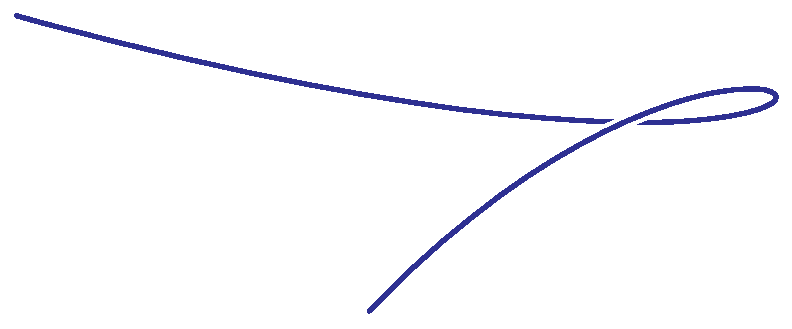
\includegraphics[height=2cm]{pictures/curve.eps}\vspace{-19pt}
\]


\noindent
\begin{tabular}{rcl}
  A cubic polynomial $f(t)$ &$\Longleftrightarrow$& 
   affine function applied to $\gamma$\\
  &$\Longleftrightarrow$& affine hyperplane, \DeCo{$f^\perp$}\\ \rule{0pt}{22pt}
  Two polynomials $f,g$ &$\Longleftrightarrow$& two affine hyperplanes\\
            &$\Longleftrightarrow$& a line 
   \DeCo{$f^\perp\cap g^\perp$}\\
   \rule{0pt}{25pt}
  $\Wr(f,g)(s)=0$ &$\Longleftrightarrow$& the line 
  $f^\perp\cap g^\perp$
   meets \\
  && tangent line to $\gamma$ at $\gamma(s)$. \\   \rule{0pt}{45pt}
  \begin{minipage}[c]{5cm}
  $\Wr(f,g)$ is a given quartic $F$
  \end{minipage}
  &$\Longleftrightarrow$& 
  \begin{minipage}[c]{8cm}
   $f^\perp\cap g^\perp$
   meets tangents to $\gamma$
   at the four roots of $F$
  \end{minipage}
\end{tabular}


%%%%%%%%%%%%%%%%%%%%%%%%%%%%%%%%%%%%%%%%%%%%%%%%%%%%%%%%%%%%%%


%%%%%%%%%%%%%%%%%%%%%%%%%%%%%%%%%%%%%%%%%%%%%%%%%%%%%%%%%%%%%%
\slide{}
\LogoOn
\begin{center}
\RawSienna{{\LARGE }}
\end{center}


\begin{center}\rule{0pt}{150pt}
\Red{\framebox{View Animation}}
\end{center}
\thispagestyle{empty}
%%%%%%%%%%%%%%%%%%%%%%%%%%%%%%%%%%%%%%%%%%%%%%%%%%%%%%%%%%%%%%


\setcounter{page}{3}

%%%%%%%%%%%%%%%%%%%%%%%%%%%%%%%%%%%%%%%%%%%%%%%%%%%%%%%%%%%%%%
\slide{}
\LogoOn
\begin{center}
\RawSienna{{\LARGE Numerical accident ?}}
\end{center}

\noindent
The proof begins with a numerical accident.

\noindent
In 1884, Schubert (essentially) determined that 
\[
\# \Wr^{-1}(F(t))\ =\  
          \dfrac{(mp)!\,0!1!2!\dotsb {m-1}!}{p!(p{+}1)!\dotsb (p{+}m{-}1)!}\,.
\]
Call this number \DeCo{$\deg(m,p)$}.

\noindent
This number is also the dimension of the space of invariants
\[
\deg(m,p)\ \stackrel{!}{=}\ \dim \left(\left(\C^m\right)^{\otimes mp}\right)^{{\mathfrak sl}_{m}\C}\ .
\]

\noindent
Strengthening this coincidence is at the heart of our story.


%%%%%%%%%%%%%%%%%%%%%%%%%%%%%%%%%%%%%%%%%%%%%%%%%%%%%%%%%%%%%%

%%%%%%%%%%%%%%%%%%%%%%%%%%%%%%%%%%%%%%%%%%%%%%%%%%%%%%%%%%%%%%
\slide{}
\LogoOn
\begin{center}
\RawSienna{{\LARGE A remarkable function}}
\end{center}

\noindent
For $i=1,\dotsc,m$ let \DeCo{$y_i(t)$} be a polynomial of degree $ip$.
Define the \DeCo{master function}\vspace{-10pt}
\[
  \DeCo{\Phi}\ :=\ 
   \displaystyle \prod_{i=1}^m \mbox{\sf Discr}(y_i) \Bigg/
   \displaystyle \prod_{i=1}^{m-1} \mbox{\sf Res}(y_{i},y_{i+1})\ ,  \vspace{-10pt}
\]
where \DeCo{$\mbox{\sf Discr}$} and \DeCo{$\mbox{\sf Res}$} are the classical discriminant
and resultant.\vspace{-5pt}

\noindent
Writing $\Phi$ in terms of the roots $s_{i,j}$ of $y_i$ gives,  \vspace{-5pt}
\[
  \Phi(s)\ =\ \prod_{i=1}^m\prod_{j\neq k}(s_{i,j}-s_{i,k})^{\Red{2}} \cdot
           \prod_{i=1}^{m-1}\prod_{j, k}(s_{i,j}-s_{i+1,k})^{\Red{-1}}\ . \vspace{-5pt}
\]
(The exponents come from the Cartan matrix of type $A$.)

\noindent
Remarkably, \Magenta{$\deg(m,p)$} counts the (orbits of) critical points of $\Phi(s)$.
%%%%%%%%%%%%%%%%%%%%%%%%%%%%%%%%%%%%%%%%%%%%%%%%%%%%%%%%%%%%%%

%%%%%%%%%%%%%%%%%%%%%%%%%%%%%%%%%%%%%%%%%%%%%%%%%%%%%%%%%%%%%%
\slide{}
\LogoOn
\begin{center}
\RawSienna{{\LARGE Schematic of proof}}
\end{center}

\quad
\begin{picture}(420,300)(-10,5)\thicklines 

\put(130,280){Critical points of $\Phi$}
%\put(150,265){\vector(-2,-3){80}}\put(255,265){\vector(2,-3){80}}

%\put(30,220){Fuchsian}\put(30,202){diff.~eq.}

%\put(310,220){Bethe}\put(315,202){Ansatz}

%\put(  0,115){$\Wr^{-1}(y_m(t))$}
%\put(125,120){\vector(-1,0){20}}\put(135,120){\line(1,0){20}}
%\put(175,120){\line(1,0){20}}\put(215,120){\line(1,0){20}}
%\put(255,120){\line(1,0){20}}\put(290,120){\vector(1,0){20}}
%\put(315,115){Rep. Theory}

%\put(140,130){\Magenta{! new connection}}

%\put(355,60){\vector(0,1){45}}
%\put(295,42){Eigenvalues of a}
%\put(295,23){symmetric matrix}
%\put(300,0){\Magenta{(forces reality)}}

%\put(285,30){\vector(-1,0){150}}

%\put(5,42){Real spaces}
%\put(5,23){of polynomials}
%\put(0, 0){($\Wr^{-1}(y_m(t))$) \DeCo{\raisebox{-1pt}{\rule{7pt}{14pt}}}}
\end{picture}

%%%%%%%%%%%%%%%%%%%%%%%%%%%%%%%%%%%%%%%%%%%%%%%%%%%%%%%%%%%%%%
%%%%%%%%%%%%%%%%%%%%%%%%%%%%%%%%%%%%%%%%%%%%%%%%%%%%%%%%%%%%%%

%%%%%%%%%%%%%%%%%%%%%%%%%%%%%%%%%%%%%%%%%%%%%%%%%%%%%%%%%%%%%%
\slide{}
\setcounter{page}{6}
\LogoOn
\begin{center}
\RawSienna{{\LARGE Schematic of proof}}
\end{center}

\quad
\begin{picture}(420,300)(-10,5)\thicklines 

\put(130,280){Critical points of $\Phi$}
\put(150,265){\vector(-2,-3){80}}\put(255,265){\vector(2,-3){80}}

\put(30,220){Fuchsian}\put(30,202){diff.~eq.}

\put(310,220){Bethe}\put(315,202){Ansatz}

\put(  0,115){$\Wr^{-1}(y_m(t))$}
%\put(125,120){\vector(-1,0){20}}\put(135,120){\line(1,0){20}}
%\put(175,120){\line(1,0){20}}\put(215,120){\line(1,0){20}}
%\put(255,120){\line(1,0){20}}\put(290,120){\vector(1,0){20}}
\put(315,115){Rep. Theory}

%\put(140,130){\Magenta{! new connection}}

%\put(355,60){\vector(0,1){45}}
%\put(295,42){Eigenvalues of a}
%\put(295,23){symmetric matrix}
%\put(300,0){\Magenta{(forces reality)}}

%\put(285,30){\vector(-1,0){150}}

%\put(5,42){Real spaces}
%\put(5,23){of polynomials}
%\put(0, 0){($\Wr^{-1}(y_m(t))$) \DeCo{\raisebox{-1pt}{\rule{7pt}{14pt}}}}
\end{picture}

%%%%%%%%%%%%%%%%%%%%%%%%%%%%%%%%%%%%%%%%%%%%%%%%%%%%%%%%%%%%%%

%%%%%%%%%%%%%%%%%%%%%%%%%%%%%%%%%%%%%%%%%%%%%%%%%%%%%%%%%%%%%%
\slide{}
\setcounter{page}{6}
\LogoOn
\begin{center}
\RawSienna{{\LARGE Schematic of proof}}
\end{center}

\quad
\begin{picture}(420,300)(-10,5)\thicklines 

\put(130,280){Critical points of $\Phi$}
\put(150,265){\vector(-2,-3){80}}\put(255,265){\vector(2,-3){80}}

\put(30,220){Fuchsian}\put(30,202){diff.~eq.}

\put(310,220){Bethe}\put(315,202){Ansatz}

\put(  0,115){$\Wr^{-1}(y_m(t))$}
\put(130,120){\vector(-1,0){20}}\put(145,120){\line(1,0){20}}
\put(180,120){\line(1,0){20}}\put(215,120){\line(1,0){20}}
\put(250,120){\line(1,0){20}}\put(285,120){\vector(1,0){20}}
\put(315,115){Rep. Theory}

\put(140,130){\Magenta{! new connection}}

%\put(355,60){\vector(0,1){45}}
%\put(295,42){Eigenvalues of a}
%\put(295,23){symmetric matrix}
%\put(300,0){\Magenta{(forces reality)}}

%\put(285,30){\vector(-1,0){150}}

%\put(5,42){Real spaces}
%\put(5,23){of polynomials}
%\put(0, 0){($\Wr^{-1}(y_m(t))$) \DeCo{\raisebox{-1pt}{\rule{7pt}{14pt}}}}
\end{picture}

%%%%%%%%%%%%%%%%%%%%%%%%%%%%%%%%%%%%%%%%%%%%%%%%%%%%%%%%%%%%%%


%%%%%%%%%%%%%%%%%%%%%%%%%%%%%%%%%%%%%%%%%%%%%%%%%%%%%%%%%%%%%%
\slide{}
\setcounter{page}{6}
\LogoOn
\begin{center}
\RawSienna{{\LARGE Schematic of proof}}
\end{center}

\quad
\begin{picture}(420,300)(-10,5)\thicklines 

\put(130,280){Critical points of $\Phi$}
\put(150,265){\vector(-2,-3){80}}\put(255,265){\vector(2,-3){80}}

\put(30,220){Fuchsian}\put(30,202){diff.~eq.}

\put(310,220){Bethe}\put(315,202){Ansatz}

\put(  0,115){$\Wr^{-1}(y_m(t))$}
\put(130,120){\vector(-1,0){20}}\put(145,120){\line(1,0){20}}
\put(180,120){\line(1,0){20}}\put(215,120){\line(1,0){20}}
\put(250,120){\line(1,0){20}}\put(285,120){\vector(1,0){20}}
\put(315,115){Rep. Theory}

\put(140,130){\Magenta{! new connection}}

\put(353,60){\vector(0,1){45}}
\put(298,42){Eigenvalues of a}
\put(295,23){symmetric matrix}
\put(306,0){\Magenta{(forces reality)}}

%\put(285,30){\vector(-1,0){155}}

%\put(5,42){Real spaces}
%\put(5,23){of polynomials}
%\put(0, 0){($\Wr^{-1}(y_m(t))$) \DeCo{\raisebox{-1pt}{\rule{7pt}{14pt}}}}
\end{picture}

%%%%%%%%%%%%%%%%%%%%%%%%%%%%%%%%%%%%%%%%%%%%%%%%%%%%%%%%%%%%%%


%%%%%%%%%%%%%%%%%%%%%%%%%%%%%%%%%%%%%%%%%%%%%%%%%%%%%%%%%%%%%%
\slide{}
\setcounter{page}{6}
\LogoOn
\begin{center}
\RawSienna{{\LARGE Schematic of proof}}
\end{center}

\quad
\begin{picture}(420,300)(-10,5)\thicklines 

\put(130,280){Critical points of $\Phi$}
\put(150,265){\vector(-2,-3){80}}\put(255,265){\vector(2,-3){80}}

\put(30,220){Fuchsian}\put(30,202){diff.~eq.}

\put(310,220){Bethe}\put(315,202){Ansatz}

\put(  0,115){$\Wr^{-1}(y_m(t))$}
\put(130,120){\vector(-1,0){20}}\put(145,120){\line(1,0){20}}
\put(180,120){\line(1,0){20}}\put(215,120){\line(1,0){20}}
\put(250,120){\line(1,0){20}}\put(285,120){\vector(1,0){20}}
\put(315,115){Rep. Theory}

\put(140,130){\Magenta{! new connection}}

\put(353,60){\vector(0,1){45}}
\put(298,42){Eigenvalues of a}
\put(295,23){symmetric matrix}
\put(306,0){\Magenta{(forces reality)}}

\put(283,28){\vector(-1,0){160}}

\put(5,42){Real spaces}
\put(5,23){of polynomials}
\put(0, 0){\Magenta{$\bigl(\Wr^{-1}(y_m(t))\bigr)$}}
\end{picture}

%%%%%%%%%%%%%%%%%%%%%%%%%%%%%%%%%%%%%%%%%%%%%%%%%%%%%%%%%%%%%%


%%%%%%%%%%%%%%%%%%%%%%%%%%%%%%%%%%%%%%%%%%%%%%%%%%%%%%%%%%%%%%
\slide{}
\setcounter{page}{6}
\LogoOn
\begin{center}
\RawSienna{{\LARGE Schematic of proof}}
\end{center}

\quad
\begin{picture}(420,300)(-10,5)\thicklines 

\put(130,280){Critical points of $\Phi$}
\put(150,265){\vector(-2,-3){80}}\put(255,265){\vector(2,-3){80}}

\put(30,220){Fuchsian}\put(30,202){diff.~eq.}

\put(310,220){Bethe}\put(315,202){Ansatz}

\put(  0,115){$\Wr^{-1}(y_m(t))$}
\put(130,120){\vector(-1,0){20}}\put(145,120){\line(1,0){20}}
\put(180,120){\line(1,0){20}}\put(215,120){\line(1,0){20}}
\put(250,120){\line(1,0){20}}\put(285,120){\vector(1,0){20}}
\put(315,115){Rep. Theory}

\put(140,130){\Magenta{! new connection}}

\put(353,60){\vector(0,1){45}}
\put(298,42){Eigenvalues of a}
\put(295,23){symmetric matrix}
\put(306,0){\Magenta{(forces reality)}}

\put(283,28){\vector(-1,0){160}}

\put(5,42){Real spaces}
\put(5,23){of polynomials}
\put(0, 0){\Magenta{$\bigl(\Wr^{-1}(y_m(t))\bigr)$} \DeCo{\raisebox{-3pt}{\rule{9pt}{18pt}}}}
\end{picture}

%%%%%%%%%%%%%%%%%%%%%%%%%%%%%%%%%%%%%%%%%%%%%%%%%%%%%%%%%%%%%%

%%%%%%%%%%%%%%%%%%%%%%%%%%%%%%%%%%%%%%%%%%%%%%%%%%%%%%%%%%%%%%
\slide{}
\LogoOn
\begin{center}
\RawSienna{{\LARGE Critical points of master function}}
\end{center}

\noindent
For $i=1,\dotsc,m$, let \DeCo{$y_i(t)$} be a polynomial of degree $ip$.
Recall the \DeCo{master function}\vspace{-10pt}
\[
  \DeCo{\Phi}\ :=\ 
   \displaystyle \prod_{i=1}^m \mbox{\sf Discr}(y_i) \Bigg/
   \displaystyle \prod_{i=1}^{m-1} \mbox{\sf Res}(y_{i},y_{i+1})\ .  \vspace{-20pt}
\]

\noindent
Fix $y_m(t)$ to be a polynomial of degree $mp$
with roots $\DeCo{\bs}:=(s_1,\dotsc,s_{mp})$.
This will be our Wronski polynomial. 

\noindent
The master function \DeCo{$\Phi_\bs(\bx)$} depends on the roots $\bx$ of the other
$y_i$. 

\noindent
Let \DeCo{$\bx$} be a critical point of $\Phi_\bs(\bx)$, and 
$\DeCo{\by}:=(y_1,\dotsc,y_{m-1})$ the corresponding polynomials whose roots are $\bx$.

\noindent
\Purple{Theorem.} \Brown{(MV)}
{\sl There are $\deg(m,p)$ such critical points $\by$.}

%%%%%%%%%%%%%%%%%%%%%%%%%%%%%%%%%%%%%%%%%%%%%%%%%%%%%%%%%%%%%%

%%%%%%%%%%%%%%%%%%%%%%%%%%%%%%%%%%%%%%%%%%%%%%%%%%%%%%%%%%%%%%
\slide{}
\LogoOn
\begin{center}
\RawSienna{{\LARGE Spaces of polynomials from $\by$}}
\end{center}

\noindent
For polynomials $\by=(y_1,\dotsc,y_{m-1})$, with $\deg y_i=ip$,\newline
the \DeCo{{\sl fundamental differential operator} $D_{\by}$} is
\[
  \bigl(\tfrac{d}{dt}-\ln'\bigl(\tfrac{y_m}{y_{m-1}}\bigr)\bigr)
   \dotsb
  \bigl(\tfrac{d}{dt}-\ln'\bigl(\tfrac{y_1}{y_1}\bigr)\bigr)
  \bigl(\tfrac{d}{dt}-\ln'\bigl(y_1\bigr)\bigr)\ .
\]
 Let \DeCo{$V_\by$} be the kernel of $D_\by$.\vspace{5pt}

\noindent\Purple{Theorem.} \Brown{(MV)}\ \vspace{-20pt}
{\sl 
 \begin{enumerate}
  \item
   $V_\by$ is a space of polynomials iff $\by$ is a critical point of $\Phi_\bs$.
  \item
   If $f_1,\dotsc,f_m$ span $V_\by$ with $\deg f_i=p{+}i$, then\vspace{-5pt}
  \[
   \begin{array}{rcl}
    y_1&=& f_1\,,\\
    y_2&=& \Wr(f_1,f_2)\,,\\
       &\vdots&\\
    y_m&=& \Wr(f_1,f_2,\dotsc,f_m)\,.
  \end{array}
\]
 \end{enumerate}
}
%%%%%%%%%%%%%%%%%%%%%%%%%%%%%%%%%%%%%%%%%%%%%%%%%%%%%%%%%%%%%%

%%%%%%%%%%%%%%%%%%%%%%%%%%%%%%%%%%%%%%%%%%%%%%%%%%%%%%%%%%%%%%
\slide{}
\LogoOn
\begin{center}
\RawSienna{{\LARGE Finite-dimensional $\mathfrak{sl}_{m}\C$-modules}}
\end{center}

\noindent
Finite-dimensional  $\mathfrak{sl}_{m}\C$-modules $V$ are sum of 
\DeCo{{\sl weight spaces} $V[\mu]$}.

\noindent 
The \DeCo{{\sl singular vectors}}, \DeCo{sing$V[\mu]$}, in $V[\mu]$ are those annihilated
by $\mathfrak{n}^+$.

\noindent
We have the direct sum decomposition
\[
     V\ =\ \bigoplus_\mu U\mathfrak{sl}_{m}\C.\mbox{sing}V[\mu]\,,\vspace{-5pt}
\]
where \DeCo{$U\mathfrak{sl}_{m}\C$} is the universal enveloping algebra.

\noindent
Each singular vector generates an irreducible summand of $V$.

\noindent
Consequently, finding a basis of the singular vectors decomposes $V$ into irreducible
submodules.

%%%%%%%%%%%%%%%%%%%%%%%%%%%%%%%%%%%%%%%%%%%%%%%%%%%%%%%%%%%%%%


%%%%%%%%%%%%%%%%%%%%%%%%%%%%%%%%%%%%%%%%%%%%%%%%%%%%%%%%%%%%%%
\slide{}
\LogoOn
\begin{center}
\RawSienna{{\LARGE Periodic Gaudin model}}
\end{center}

\noindent$\DeCo{V}:=$ dual of vector representation of $\mathfrak{sl}_{m}\C$ 
 (also $\mathfrak{gl}_{m}\C$).\vspace{-12pt}

\noindent
Let \DeCo{$e_{i,j}\in\mathfrak{gl}_{m}\C$} be the elementary matrix with 1 
in $i,j$ position.

\noindent
Define an operator \vspace{2pt}
${\displaystyle\DeCo{X_{i,j}(t)}\ := 
  \delta_{i,j}\frac{d}{dt}\ -\ \sum_{k=1}^{mp}\frac{e_{i,j}^{(k)}}{t-s_k}}$\,,
\newline
where $e_{i,j}^{(k)}$ acts on the  $k$th factor in $V^{\otimes mp}$.

\noindent
\Magenta{Formal conjugate} of the expansion of the \Red{row} determinant of
$(X_{i,j})$ is
\[
   \frac{d^{m}}{dt^{m}} 
 + K_1(t)\frac{d^{m-1}}{dt^{m-1}}+\dotsb+K_{m-1}(t)\frac{d}{dt}+K_{m}(t)\,.
\]
$K_1(t),\dotsc,K_{m}(t)$ are the \DeCo{Gaudin Hamiltonians}.
They form a family of commuting operators on $V^{\otimes mp}$,
centralizing $\mathfrak{gl}_{m}\C$.


%%%%%%%%%%%%%%%%%%%%%%%%%%%%%%%%%%%%%%%%%%%%%%%%%%%%%%%%%%%%%%


%%%%%%%%%%%%%%%%%%%%%%%%%%%%%%%%%%%%%%%%%%%%%%%%%%%%%%%%%%%%%%
\slide{}
\LogoOn
\begin{center}
\RawSienna{{\LARGE Bethe Ansatz for Gaudin model}}
\end{center}

\noindent
In the theory of integrable systems, 
\DeCo{Bethe Ans\"atze} are conjectural methods to find the joint eigenvectors and spectra
of families of commuting operators.

\noindent
As the Gaudin Hamiltonians centralize the action of $\mathfrak{sl}_{m}\C$,\vspace{4pt}
% on $V^{\otimes mp}$,  
the Bethe Ansatz also gives a precise way to
understand $\left(V^{\otimes mp}\right)^{\mathfrak{sl}_{m}\C}$.\vspace{-5pt}

\noindent
The idea is to define a (rational) \DeCo{universal weight function}\vspace{-5pt}
\[
   \beta\ \colon\ 
   \raisebox{-10pt}{\begin{minipage}[c]{4.9cm}
    \ spaces of roots of\vspace{-5pt}\newline
    $\underbrace{y_1,\dotsc,y_{m-1}}_{\mbox{\normalsize$\bx$}}\,,
      \,\underbrace{y_m}_{\mbox{\normalsize$\bs$}}$
   \end{minipage}}\ 
    \ \longrightarrow\ \ \mbox{$0$-weight space of $V^{\otimes mp}$}\,,
\]
and then address for which values $(\bx,\bs)$ is $\beta(\bx,\bs)$ 
$\mathfrak{sl}_{m}\C$-invariant.


%%%%%%%%%%%%%%%%%%%%%%%%%%%%%%%%%%%%%%%%%%%%%%%%%%%%%%%%%%%%%%


%%%%%%%%%%%%%%%%%%%%%%%%%%%%%%%%%%%%%%%%%%%%%%%%%%%%%%%%%%%%%%
\slide{}
\LogoOn
\begin{center}
\RawSienna{{\LARGE Completeness of the Bethe Ansatz}}\vspace{-2pt}
\end{center}


\noindent\Purple{{\large Theorem.}} \Brown{(MTV)}
{\sl
   Let $\bx$ be a critical point of the master function $\Phi_\bs$.\vspace{-17pt}
\begin{enumerate}
  \item $\beta(\bx,\bs)$ is well-defined, non-zero, and a joint eigenvector of 
         the Gaudin Hamiltonians.
  \item $\beta(\bx,\bs)$ is a $\mathfrak{sl}_{m}\C$-invariant.
  \item When $\bs$ is general, the vectors $\beta(\bx,\bs)$ for $\bx$ a critical point
    form a basis of $\bigl(V^{\otimes mp}\bigr)^{\mathfrak{sl}_{m}\C}$.
  \item When $\bs$ is general, the Gaudin Hamiltonians have simple spectrum.
  \item The eigenvalues \DeCo{$\lambda_i(t)$} of $K_i(t)$ on $\beta(\bx,\bs)$
    satisfy\vspace{-12pt} 
\begin{multline*}
  \frac{d^{m}}{dt^{m}}+\lambda_1(t)\frac{d^{m-1}}{dt^{m-1}}+\dotsb+
    \lambda_{m-1}(t)\frac{d}{dt}+\lambda_{m}(t)\ =\\
   \bigl(\tfrac{d}{dt}-\ln'\bigl(\tfrac{y_m}{y_{m-1}}\bigr)\bigr)
   \dotsb
  \bigl(\tfrac{d}{dt}-\ln'\bigl(\tfrac{y_2}{y_1}\bigr)\bigr)
  \bigl(\tfrac{d}{dt}-\ln'\bigl(y_1\bigr)\bigr)\,,
\end{multline*} 
 the fundamental differential operator of the critical point $\bx$.
 \end{enumerate}
}

%%%%%%%%%%%%%%%%%%%%%%%%%%%%%%%%%%%%%%%%%%%%%%%%%%%%%%%%%%%%%%


%%%%%%%%%%%%%%%%%%%%%%%%%%%%%%%%%%%%%%%%%%%%%%%%%%%%%%%%%%%%%%
\slide{}
\LogoOn
\begin{center}
\RawSienna{{\LARGE Proof of the Shapiro Conjecture}}
\end{center}

\noindent
Usual Euclidean inner product on $V$ induces the 
\DeCo{Shapovalov form} on $V^{\otimes mp}$, which is 
$\mathfrak{sl}_{m}\C$-invariant.

\noindent
Gaudin Hamiltonians are symmetric w.r.t~the Shapovalov form.

\noindent
Therefore, when $\bs$ and $t$ are real, their eigenvalues $\lambda_i(t)$ on a vector
$\beta(\bx,\bs)$ for a critical point $\bx$ are real.

\noindent
Then the fundamental differential operator is real, and thus its kernel $V_\bx$ is also
real. 

\noindent
This implies the MTV Reality Theorem, as spaces $V_\bx$ for $\bx$ a critical point give all
spaces of polynomials whose Wronskian has roots $\bs$.
%%%%%%%%%%%%%%%%%%%%%%%%%%%%%%%%%%%%%%%%%%%%%%%%%%%%%%%%%%%%%%



%%%%%%%%%%%%%%%%%%%%%%%%%%%%%%%%%%%%%%%%%%%%%%%%%%%%%%%%%%%%%%
\slide{}
\LogoOn
\begin{center}
\RawSienna{{\LARGE Thank you for your attention!}}
\end{center}

\begin{picture}(420,300)
\put(57,42){\includegraphics[height=5cm]{pictures/frsc_fix.eps}}
\end{picture}
%%%%%%%%%%%%%%%%%%%%%%%%%%%%%%%%%%%%%%%%%%%%%%%%%%%%%%%%%%%%%%


%%%%%%%%%%%%%%%%%%%%%%%%%%%%%%%%%%%%%%%%%%%%%%%%%%%%%%%%%%%%%%

\end{document}
